% --- Вопрос 26 ---
\examquestion{26}{Длина дуги гладкой кривой}
{Сформулируйте теорему о длине дуги гладкой кривой, заданной уравнением $y = y(x), x \in [a, b]$, где $y'(x) \in C[a, b]$. Проведите доказательство этой формулы, используя определение предела длин вписанных ломаных. На этапе преобразования приращений координат $\Delta y_i$ строго примените теорему Лагранжа о конечном приращении и критерий интегрируемости Римана.}

\paragraph{Суть на пальцах}
Прямую линейку к кривой не приложишь. Режем кривую на куски и соединяем точки отрезками. Длину отрезка находим по теореме Пифагора. По теореме Лагранжа вертикальный катет $\Delta y$ выражаем через производную $y'$. Выносим шаг $\Delta x$ за корень. При бесконечном измельчении сумма всех гипотенуз превращается в определенный интеграл.

\paragraph{Справка: О чем теорема Лагранжа}
Теорема о конечном приращении гласит: если функция непрерывна на отрезке и дифференцируема внутри него, то между концами отрезка существует точка $c$, такая что $f(b) - f(a) = f'(c)(b - a)$. В контексте длины дуги это означает, что приращение высоты $\Delta y_i$ на любом мелком шаге можно заменить на наклон касательной в некой промежуточной точке $\xi_i$, умноженный на ширину шага $\Delta x_i$. Геометрически: на дуге всегда найдется точка, касательная в которой параллельна хорде.

\paragraph{Формулировка}
Если функция $y(x)$ непрерывно дифференцируема на отрезке $[a, b]$, то дуга этой кривой спрямляема (имеет конечную длину), и ее длина вычисляется по формуле:
$$L = \int_a^b \sqrt{1 + (y'(x))^2} dx$$

\begin{center}
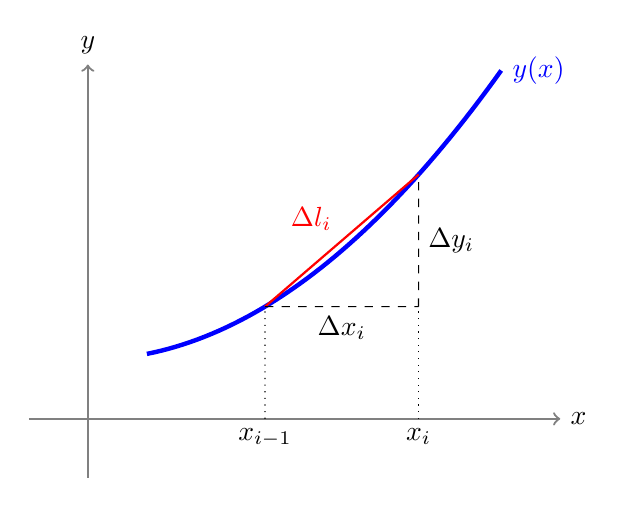
\begin{tikzpicture}[scale=1.5]
    % Оси
    \draw[->, thick, gray] (-0.5,0) -- (4,0) node[right, black] {$x$};
    \draw[->, thick, gray] (0,-0.5) -- (0,3) node[above, black] {$y$};
    
    % Кривая
    \draw[ultra thick, blue, domain=0.5:3.5, samples=50] plot (\x, {0.5 + 0.2*\x*\x}) node[right] {$y(x)$};
    
    % Точки разбиения
    \coordinate (P1) at (1.5, 0.95); % x_{i-1}
    \coordinate (P2) at (2.8, 2.068); % x_i
    
    % Ломаная (хорда)
    \draw[red, thick] (P1) -- (P2) node[midway, above left] {$\Delta l_i$};
    
    % Прямоугольный треугольник приращений
    \draw[dashed, black] (P1) -- (2.8, 0.95) node[midway, below] {$\Delta x_i$};
    \draw[dashed, black] (2.8, 0.95) -- (P2) node[midway, right] {$\Delta y_i$};
    
    % Проекции на ось X
    \draw[dotted] (1.5, 0) node[below] {$x_{i-1}$} -- (P1);
    \draw[dotted] (2.8, 0) node[below] {$x_i$} -- (2.8, 0.95);
\end{tikzpicture}
\end{center}

\begin{proof}
1. Разбиваем отрезок $[a, b]$ точками $x_i$ с шагом $\Delta x_i$. 
2. По теореме Пифагора длина $i$-го звена ломаной (хорды):
$$\Delta l_i = \sqrt{\Delta x_i^2 + \Delta y_i^2}$$
3. Так как кривая гладкая, функция $y(x)$ непрерывна и дифференцируема на каждом частичном отрезке $[x_{i-1}, x_i]$. Следовательно, по \textbf{теореме Лагранжа} внутри отрезка гарантированно найдется точка $\xi_i$, в которой приращение функции выражается через производную:
$$\Delta y_i = y'(\xi_i) \Delta x_i$$
4. Подставляем это выражение в корень и выносим общий положительный множитель $\Delta x_i$:
$$\Delta l_i = \sqrt{1 + (y'(\xi_i))^2} \Delta x_i$$
5. Суммируя длины всех звеньев, получаем интегральную сумму Римана:
$$L_n = \sum_{i=1}^n \sqrt{1 + (y'(\xi_i))^2} \Delta x_i$$
6. \textbf{Проверка интегрируемости (цепочка выводов):}
\begin{itemize}
    \item По условию производная $y'(x)$ непрерывна на $[a, b]$.
    \item Следовательно, сложная функция $\sqrt{1 + (y'(x))^2}$ также непрерывна.
    \item По критерию Римана любая непрерывная функция является интегрируемой.
\end{itemize}
7. \textbf{Переход к пределу:}
Так как функция интегрируема, при измельчении разбиения ($\lambda \to 0$) предел суммы существует, не зависит от выбора точек $\xi_i$ и переходит в определенный интеграл:
$$L = \lim_{\lambda \to 0} L_n = \int_a^b \sqrt{1 + (y'(x))^2} dx$$
Теорема доказана.
\end{proof}

% --- Для Вопроса 26 (Длина дуги гладкой кривой) ---
\begin{tcolorbox}[colback=gray!5, colframe=black, boxrule=0.5pt, arc=0pt]
\textbf{Резюмируем:} \\
\textbf{Тезис:} Дуга спрямляема, $L = \int_a^b \sqrt{1 + (y'(x))^2} dx$. \\
\textbf{Ход:} Длина звена ломаной $\Delta l_i = \sqrt{\Delta x_i^2 + \Delta y_i^2}$. По т. Лагранжа заменяем $\Delta y_i = y'(\xi_i) \Delta x_i$. \\
\textbf{Трюк:} Выносим $\Delta x_i$ за корень: $\Delta l_i = \sqrt{1 + (y'(\xi_i))^2} \Delta x_i$. Получаем интегральную сумму. \\
\textbf{Финал:} Так как $y'(x)$ непрерывна, корень тоже непрерывен. При $\lambda \to 0$ сумма Римана переходит в определенный интеграл.
\end{tcolorbox}




% --- Вопрос 27 ---
\examquestion{27}{Объемы тел вращения: методы дисков и оболочек}
{Сформулируйте и докажите теоремы о вычислении объема тела вращения криволинейной трапеции, ограниченной непрерывной функцией $y = f(x), x \in [a, b]$. Проведите выводы формул вращения вокруг оси Ox (метод дисков) и оси Oy (метод оболочек).}

\paragraph{Суть на пальцах}
Объем любой сложной фигуры можно посчитать, разрезав ее на простые куски. 
Если вращаем фигуру вокруг горизонтальной оси Ox, она становится похожа на колбасу. Режем ее поперек получаем тонкие круглые монетки (диски). Объем монетки это площадь круга на толщину $dx$.
Если вращаем фигуру вокруг вертикальной оси Oy, она похожа на цилиндрический торт. Режем ее как луковицу на слои получаем полые трубы (оболочки). Объем трубы это длина окружности на высоту и на толщину стенки $dx$.

\paragraph{(a) Метод дисков (вращение вокруг Ox)}
\begin{center}
\begin{tikzpicture}[scale=1.2]
    \draw[->, thick] (-0.5,0) -- (4,0) node[right] {$x$};
    \draw[->, thick] (0,-1.5) -- (0,2.5) node[above] {$y$};
    
    % Функция и симметричная ей
    \draw[thick, blue, domain=0.5:3.5] plot (\x, {1 + 0.3*sin(\x*50)});
    \draw[thick, blue, dashed, domain=0.5:3.5] plot (\x, {-(1 + 0.3*sin(\x*50))});
    
    % Эллипсы для объема
    \draw[gray] (0.5,0) ellipse (0.1 and {1 + 0.3*sin(0.5*50)});
    \draw[gray] (3.5,0) ellipse (0.1 and {1 + 0.3*sin(3.5*50)});
    
    % Выделенный диск
    \fill[red!20, opacity=0.8] (2.0,0) ellipse (0.15 and {1 + 0.3*sin(2.0*50)});
    \draw[red, thick] (2.0, {1 + 0.3*sin(2.0*50)}) -- (2.3, {1 + 0.3*sin(2.3*50)});
    \draw[red, thick] (2.0, {-(1 + 0.3*sin(2.0*50))}) -- (2.3, {-(1 + 0.3*sin(2.3*50))});
    
    \node[below] at (2.15, -1.3) {$dx$};
    \draw[<-] (2.0, 1.4) -- (2.5, 2.0) node[right] {Радиус $R = f(x)$};
\end{tikzpicture}
\end{center}

\textbf{Формула:} $V_x = \pi \int_a^b f^2(x) dx$

\begin{proof}
1. Разобьем отрезок $[a, b]$ точками $x_i$ на малые части $\Delta x_i$. Выберем внутри каждой части точку $\xi_i$.
2. Аппроксимируем кусок криволинейной трапеции прямоугольником шириной $\Delta x_i$ и высотой $f(\xi_i)$.
3. При вращении этого прямоугольника вокруг оси Ox получается цилиндрический диск.
4. Объем прямого цилиндра равен площади основания на высоту. Основание это круг радиуса $R = f(\xi_i)$, а высота цилиндра это наша толщина $\Delta x_i$.
$$\Delta V_i = \pi R^2 H = \pi f^2(\xi_i) \Delta x_i$$
5. Суммируем объемы всех дисков, получаем интегральную сумму:
$$V_n = \sum_{i=1}^n \pi f^2(\xi_i) \Delta x_i$$
6. Так как $f(x)$ непрерывна, $f^2(x)$ тоже непрерывна. Переходим к пределу при $\lambda \to 0$ и получаем определенный интеграл Римана:
$$V_x = \pi \int_a^b f^2(x) dx$$
\end{proof}

\paragraph{(b) Метод оболочек (вращение вокруг Oy)}
\begin{center}
\begin{tikzpicture}[scale=1.2]
    \draw[->, thick] (-0.5,0) -- (4,0) node[right] {$x$};
    \draw[->, thick] (0,-0.5) -- (0,3) node[above] {$y$};
    
    \draw[thick, blue, domain=1:3] plot (\x, {2.5 - 0.2*(\x-2)*(\x-2)});
    
    % Выделенная полоса (оболочка в разрезе)
    \draw[red, fill=red!20] (2.2, 0) rectangle (2.4, {2.5 - 0.2*(2.2-2)*(2.2-2)});
    
    \draw[dashed, gray] (2.3, 0) -- (2.3, 2.5);
    \draw[<->] (0, 0.5) -- (2.3, 0.5) node[midway, above] {Радиус $r = x$};
    
    \node[right] at (2.4, 1.2) {Высота $h = f(x)$};
    \node[below] at (2.3, 0) {$dx$};
\end{tikzpicture}
\end{center}

\textbf{Формула:} $V_y = 2\pi \int_a^b x f(x) dx$

\begin{proof}
1. Снова разбиваем отрезок $[a, b]$ на части $\Delta x_i$. Берем точку $\xi_i \in [x_{i-1}, x_i]$.
2. Аппроксимируем площадь узким прямоугольником с основанием $\Delta x_i$ и высотой $f(\xi_i)$, который отстоит от оси вращения (Oy) на расстояние $\xi_i$.
3. При вращении этого прямоугольника вокруг оси Oy он заметает в пространстве полый цилиндр (оболочку).
4. Чтобы найти объем оболочки, разрежем ее вдоль и развернем в плоский прямоугольный параллелепипед. 
   Его длина равна длине окружности $L = 2\pi r = 2\pi \xi_i$. 
   Высота равна $H = f(\xi_i)$. 
   Толщина равна $\Delta x_i$.
5. Объем одной такой оболочки:
$$\Delta V_i = (2\pi \xi_i) \cdot f(\xi_i) \cdot \Delta x_i$$
6. Суммируем по всем отрезкам разбиения:
$$V_n = \sum_{i=1}^n 2\pi \xi_i f(\xi_i) \Delta x_i$$
7. Это интегральная сумма Римана для непрерывной функции $g(x) = 2\pi x f(x)$. При $\lambda \to 0$ предел суммы дает нам точный интеграл:
$$V_y = \int_a^b 2\pi x f(x) dx = 2\pi \int_a^b x f(x) dx$$
\end{proof}

\paragraph{Бонус: Пример расчета}
Вращение параболы $y = x^2$ на $[0, 1]$ вокруг оси $Ox$:
$$V_x = \pi \int_0^1 (x^2)^2 \, dx = \pi \int_0^1 x^4 \, dx = \pi \left[ \frac{x^5}{5} \right]_0^1 = \frac{\pi}{5}$$


% --- Для Вопроса 27 (Объемы тел вращения: методы дисков и оболочек) ---
\begin{tcolorbox}[colback=gray!5, colframe=black, boxrule=0.5pt, arc=0pt]
\textbf{Резюмируем:} \\
\textbf{Тезис:} Вращение вокруг Ox (диски): $V_x = \pi \int_a^b f^2(x) dx$. Около Oy (оболочки): $V_y = 2\pi \int_a^b x f(x) dx$. \\
\textbf{Ход Ox:} Аппроксимируем объем цилиндрами. Радиус $R=f(\xi_i)$, толщина $\Delta x_i$. Объем диска $\Delta V_i = \pi f^2(\xi_i) \Delta x_i$. \\
\textbf{Ход Oy:} Оболочка — полый цилиндр. Длина $2\pi \xi_i$, высота $f(\xi_i)$, толщина $\Delta x_i \implies \Delta V_i = 2\pi \xi_i f(\xi_i) \Delta x_i$. \\
\textbf{Финал:} Функция $f(x)$ непрерывна. При мелкости разбиения $\lambda \to 0$ интегральные суммы переходят в формулы точных интегралов.
\end{tcolorbox}






% --- Вопрос 28 ---
\examquestion{28}{Признаки Дирихле и Абеля для несобственных интегралов}
{Сформулируйте признак Дирихле сходимости интеграла $\int_a^{+\infty} f(x)g(x) dx$. Опираясь на вторую теорему о среднем значении (в форме Бонне), приведите обоснование признака Дирихле. На примере интеграла Дирихле $\int_0^{+\infty} \frac{\sin x}{x} dx$ покажите классическое применение инструмента и докажите отсутствие абсолютной сходимости.}

\paragraph{Ликбез!}
\begin{itemize}
    \item \textbf{Собственный интеграл (Римана):} Считаем площадь под графиком на жестко заданном, конечном отрезке $[a, b]$. Функция там не улетает в бесконечность. Площадь всегда равна какому-то конкретному числу.
    \item \textbf{Несобственный интеграл:} Отрезок интегрирования бесконечен (от $a$ до $+\infty$). Мы пытаемся посчитать площадь фигуры, которая тянется вправо бесконечно долго.
    \item \textbf{Что значит «интеграл сходится»?} Мы считаем интеграл до конечной точки $A$, а потом устремляем $A \to +\infty$. Если предел площади конечен — это сходимость.
\end{itemize}

\paragraph{Суть на пальцах: Дирихле против Абеля}
Мы перемножаем два сигнала $f(x)$ и $g(x)$.
\begin{itemize}
    \item \textbf{Дирихле:} Первый сигнал $f(x)$ просто болтается в рамках (первообразная ограничена), но сам по себе не затухает. Тогда второй сигнал $g(x)$ обязан работать как жесткий «глушитель» — плавно уходить в ноль, чтобы их произведение успокоилось.
    \item \textbf{Абель:} Первый сигнал $f(x)$ уже сам по себе хороший (его собственный интеграл сходится). Тогда от второго сигнала $g(x)$ требуется только не испортить эту картину: он должен быть плавным (монотонным) и не улетать в бесконечность (быть ограниченным).
\end{itemize}

\paragraph{Формулировка (Признак Дирихле)}
Несобственный интеграл $\int_a^{+\infty} f(x)g(x) dx$ сходится, если:
\begin{enumerate}
    \item Функция $f(x)$ имеет на $[a, +\infty)$ ограниченную первообразную: $\exists M > 0, \forall A > a : \left| \int_a^A f(x) dx \right| \le M$.
    \item Функция $g(x)$ монотонно стремится к нулю при $x \to +\infty$.
\end{enumerate}

\paragraph{Формулировка (Признак Абеля)}
Несобственный интеграл $\int_a^{+\infty} f(x)g(x) dx$ сходится, если:
\begin{enumerate}
    \item Интеграл $\int_a^{+\infty} f(x) dx$ сходится.
    \item Функция $g(x)$ монотонна и ограничена на $[a, +\infty)$.
\end{enumerate}

\begin{proof}[Доказательство признака Дирихле (через теорему Бонне)]
1. Воспользуемся критерием Коши для несобственных интегралов. Нам нужно доказать, что для любого $\varepsilon > 0$ найдется такое $R$, что для любых $A, B > R$ кусок площади на бесконечности пренебрежимо мал: $\left| \int_A^B f(x)g(x) dx \right| < \varepsilon$. \\
2. Так как $g(x)$ монотонна и стремится к нулю, применим вторую теорему о среднем значении (в форме Бонне) на отрезке $[A, B]$. По ней существует точка $\xi \in [A, B]$, такая что:
$$\int_A^B f(x)g(x) dx = g(A) \int_A^\xi f(x) dx$$
(так как $g(x) \to 0$, второе классическое слагаемое с $g(B)$ отпадает). \\
3. Оценим интеграл от $f(x)$. Так как первообразная ограничена числом $M$:
$$\left| \int_A^\xi f(x) dx \right| = \left| \int_a^\xi f(x) dx - \int_a^A f(x) dx \right| \le M + M = 2M$$
4. Тогда весь модуль интеграла оценивается как:
$$\left| \int_A^B f(x)g(x) dx \right| \le 2M \cdot |g(A)|$$
5. Поскольку $g(x) \to 0$ при $x \to +\infty$, мы можем уйти так далеко вправо (выбрать такое большое $A$), что $|g(A)| < \frac{\varepsilon}{2M}$. \\
6. Тогда $\left| \int_A^B f(x)g(x) dx \right| < \varepsilon$. Критерий Коши выполнен, интеграл сходится.
\end{proof}

\paragraph{Пример: Интеграл Дирихле $\int_0^{+\infty} \frac{\sin x}{x} dx$}
В точке $x=0$ подынтегральная функция не определена, но $\lim_{x \to 0} \frac{\sin x}{x} = 1$. Особенности в нуле нет (она устранимая). Поэтому разобьем интеграл:
$$\int_0^{+\infty} \frac{\sin x}{x} dx = \int_0^1 \frac{\sin x}{x} dx + \int_1^{+\infty} \frac{\sin x}{x} dx$$
Первый интеграл на $[0, 1]$ является обычным \textbf{собственным интегралом} Римана (конечное число). Судьбу всей суммы решает несобственный хвост от $1$ до $+\infty$.
\begin{itemize}
    \item \textbf{Сходимость:} Пусть $f(x) = \sin x$ и $g(x) = \frac{1}{x}$. Первообразная синуса это $-\cos x$, она ограничена ($|\cos x| \le 1 \implies M=2$). Множитель $\frac{1}{x}$ монотонно стремится к нулю. По признаку Дирихле несобственный хвост сходится.
    \item \textbf{Отсутствие абсолютной сходимости:} Рассмотрим интеграл от модуля $\int_1^{+\infty} \frac{|\sin x|}{x} dx$. 
    Используем неравенство $|\sin x| \ge \sin^2 x = \frac{1 - \cos 2x}{2}$:
    $$\int_1^{+\infty} \frac{|\sin x|}{x} dx \ge \frac{1}{2} \int_1^{+\infty} \frac{1}{x} dx - \frac{1}{2} \int_1^{+\infty} \frac{\cos 2x}{x} dx$$
    Первый интеграл (гармонический) расходится к $+\infty$. Второй сходится по признаку Дирихле. Сумма расходящегося и сходящегося интегралов расходится. Значит, сам интеграл сходится, но интеграл от его модуля — расходится (абсолютной сходимости нет).
\end{itemize}

% --- Для Вопроса 28 (Признаки Дирихле и Абеля для несобственных интегралов) ---
\begin{tcolorbox}[colback=gray!5, colframe=black, boxrule=0.5pt, arc=0pt]
\textbf{Резюмируем:} \\
\textbf{Тезис:} Дирихле: первообразная $\int f$ ограничена числом $M$, $g(x) \searrow 0$. Абель: $\int f$ сходится, $g(x)$ монотонна и ограничена. \\
\textbf{Ход (Дирихле):} Оцениваем хвост по критерию Коши $\int_A^B fg dx$. По т. Бонне это $g(A) \int_A^\xi f dx$. \\
\textbf{Трюк:} Из ограниченности первообразной $\left| \int_A^\xi f dx \right| \le 2M$. Весь модуль $\le 2M \cdot |g(A)|$. \\
\textbf{Финал:} Так как $g(x) \to 0$, можно выбрать большое $A$, чтобы хвост стал $< \varepsilon$. Пример: $\int \frac{\sin x}{x} dx$ сходится по Дирихле, но не абсолютно.
\end{tcolorbox}

% --- Вопрос 29 ---
\examquestion{29}{Определение числового ряда и необходимый признак сходимости}
{Сформулируйте определение сходимости ряда через предел последовательности частичных сумм. Сформулируйте и докажите теорему о необходимом признаке сходимости. На примере гармонического ряда покажите, что стремление общего члена к нулю не влечет сходимость.}

\paragraph{Суть на пальцах}
Ряд — это бесконечная сумма чисел. Чтобы её посчитать, мы складываем элементы по одному и смотрим на «промежуточный итог» (частичную сумму). Если этот итог со временем замирает около одного конкретного числа — ряд сходится. 
Логично, что если общая сумма конечна, то те кусочки, которые мы прибавляем на бесконечности, должны быть практически нулевыми (необходимый признак). Но осторожно: сами по себе нулевые кусочки не гарантируют конечную сумму! Можно бесконечно долго прибавлять пылинки и в итоге собрать гору размером с Эверест.

\paragraph{Формулировки}
\textbf{Определение:} Числовой ряд $\sum_{n=1}^\infty a_n$ называется \textit{сходящимся}, если существует конечный предел последовательности его частичных сумм $S_n = \sum_{k=1}^n a_k$ при $n \to \infty$. Этот предел называется суммой ряда $S$. \\
\textbf{Необходимый признак:} Если ряд $\sum_{n=1}^\infty a_n$ сходится, то его общий член стремится к нулю: $\lim_{n \to \infty} a_n = 0$.

\begin{proof}[Доказательство необходимого признака]
1. По определению сходимости ряда, предел частичных сумм существует и равен конечному числу $S$:
$$\lim_{n \to \infty} S_n = S$$
2. Выразим $n$-й член ряда через разность двух соседних частичных сумм:
$$a_n = S_n - S_{n-1}$$
3. Перейдем к пределу при $n \to \infty$. Так как пределы обеих сумм равны $S$:
$$\lim_{n \to \infty} a_n = \lim_{n \to \infty} (S_n - S_{n-1}) = \lim_{n \to \infty} S_n - \lim_{n \to \infty} S_{n-1} = S - S = 0$$
Теорема доказана.
\end{proof}

\paragraph{Пример-контрпример (Гармонический ряд)}
Рассмотрим ряд $\sum_{n=1}^\infty \frac{1}{n} = 1 + \frac{1}{2} + \frac{1}{3} + \dots$ 
Его общий член $a_n = \frac{1}{n}$ очевидно стремится к нулю при $n \to \infty$. Необходимый признак выполнен. Однако сам ряд \textbf{расходится} (его сумма равна бесконечности). Это доказывает, что стремление к нулю — это необходимое, но недостаточное условие сходимости.
% --- Для Вопроса 29 (Определение числового ряда и необходимый признак сходимости) ---
\begin{tcolorbox}[colback=gray!5, colframe=black, boxrule=0.5pt, arc=0pt]
\textbf{Резюмируем:} \\
\textbf{Тезис:} Ряд сходится, если существует конечный $\lim S_n = S$. Необходимый признак: $\lim a_n = 0$. \\
\textbf{Ход:} Выражаем $n$-й член ряда как разность частичных сумм: $a_n = S_n - S_{n-1}$. \\
\textbf{Трюк:} Переходим к пределу: $\lim a_n = \lim S_n - \lim S_{n-1} = S - S = 0$. \\
\textbf{Финал:} Стремление $a_n \to 0$ не влечет сходимость. В гармоническом ряде $\sum \frac{1}{n}$ предел равен 0, но ряд расходится.
\end{tcolorbox}


% --- Вопрос 30 ---
\examquestion{30}{Критерий Коши для сходимости числового ряда}
{Сформулируйте и проведите доказательство критерия Коши для числовых рядов, опираясь на фундаментальность последовательности частичных сумм. Обоснуйте расходимость гармонического ряда путем выбора приращения $p=n$ для оценки снизу.}

\paragraph{Суть на пальцах}
Критерий Коши — это внутренний детектор сходимости, которому вообще не нужно знать итоговую сумму ряда. Он говорит: если ряд сходится, то любой «кусок» ряда, взятый где-то очень далеко на бесконечности (сумма от $n$-го до $n+p$-го элемента), должен быть пренебрежимо мал. Если мы можем залезть в бесконечность и наскрести там кусок, который в сумме больше какого-то конкретного числа — ряд точно улетает в космос (расходится).

\paragraph{Формулировка (Критерий Коши)}
Числовой ряд $\sum_{n=1}^\infty a_n$ сходится тогда и только тогда, когда для любого $\varepsilon > 0$ существует такой номер $N$, что для всех $n > N$ и для любого натурального $p > 0$ выполняется неравенство:
$$|S_{n+p} - S_n| = |a_{n+1} + a_{n+2} + \dots + a_{n+p}| < \varepsilon$$

\begin{proof}[Доказательство]
Ряд $\sum a_n$ сходится по определению $\iff$ сходится последовательность его частичных сумм $\{S_n\}$. 
По фундаментальной теореме матанализа (Критерий Коши для последовательностей), последовательность сходится тогда и только тогда, когда она является фундаментальной.
Фундаментальность $\{S_n\}$ означает, что $\forall \varepsilon > 0$, $\exists N$, $\forall n > N, \forall p > 0$:
$$|S_{n+p} - S_n| < \varepsilon$$
Подставляя $S_{n+p} - S_n = \sum_{k=1}^{n+p} a_k - \sum_{k=1}^n a_k = a_{n+1} + \dots + a_{n+p}$, получаем в точности требуемое утверждение.
\end{proof}

\paragraph{Применение к гармоническому ряду}
Докажем строго расходимость гармонического ряда $\sum_{n=1}^\infty \frac{1}{n}$, используя отрицание критерия Коши. Нам нужно найти такое фиксированное $\varepsilon > 0$, что как бы далеко мы ни зашли (для любого $n$), всегда можно будет найти такой кусок (хвост) длиной $p$, сумма которого больше $\varepsilon$.

Выберем длину хвоста $p = n$. Тогда исследуемый кусок ряда выглядит так:
$$|S_{2n} - S_n| = \frac{1}{n+1} + \frac{1}{n+2} + \dots + \frac{1}{n+n}$$
В этой сумме ровно $n$ слагаемых. Самое маленькое из них — последнее $\left(\frac{1}{2n}\right)$.
Заменим все $n$ слагаемых на самое маленькое, чтобы получить оценку снизу (сумма уменьшится):
$$|S_{2n} - S_n| > \underbrace{\frac{1}{2n} + \frac{1}{2n} + \dots + \frac{1}{2n}}_{n \text{ раз}} = n \cdot \frac{1}{2n} = \frac{1}{2}$$
Красиво? Красиво.
Мы получили, что для любого $n$ кусок ряда длиной $p=n$ всегда строго больше $\frac{1}{2}$. Положив $\varepsilon = \frac{1}{2}$, мы видим, что критерий Коши нарушается. Следовательно, гармонический ряд расходится.

% --- Для Вопроса 30 (Критерий Коши для сходимости числового ряда) ---
\begin{tcolorbox}[colback=gray!5, colframe=black, boxrule=0.5pt, arc=0pt]
\textbf{Резюмируем:} \\
\textbf{Тезис:} Сходится $\iff \forall \varepsilon > 0 \ \exists N \ \forall n>N, \forall p>0: |a_{n+1} + \dots + a_{n+p}| < \varepsilon$. \\
\textbf{Ход:} Ряд сходится $\iff$ последовательность $\{S_n\}$ фундаментальна: $|S_{n+p} - S_n| < \varepsilon$. \\
\textbf{Трюк (Гармонический):} Берем кусок $p=n$. Тогда $|S_{2n} - S_n| = \frac{1}{n+1} + \dots + \frac{1}{2n}$ (всего $n$ слагаемых). \\
\textbf{Финал:} Заменяем все слагаемые на самое маленькое $\frac{1}{2n}$. Сумма $> n \cdot \frac{1}{2n} = 1/2$. Для $\varepsilon = 1/2$ критерий нарушен, ряд расходится.
\end{tcolorbox}